\documentclass[a4paper,11pt]{article}
\pdfoutput=1

\usepackage{jheppub}
\usepackage[T1]{fontenc}

\newcommand{\alphas}{\alpha_{S}}

\title{Including EW and mixed QCD-EW corrections into PDF fits}

\author[a,b]{S. Carrazza,}
\author[b]{E. Nocera,}
\author[a]{C. Schwan}
\author[a,b]{and M. Zaro}

\affiliation[a]{Tif Lab, Dipartimento di Fisica, Universit\`a di Milano and INFN, Sezione di Milano, 20133 Milano, Italy}
\affiliation[b]{Nikhef Theory Group, Science Park 105, 1098 XG Amsterdam, The Netherlands}

\emailAdd{stefano.carrazza@mi.infn.it}
\emailAdd{e.nocera@nikhef.nl}
\emailAdd{christopher.schwan@mi.infn.it}
\emailAdd{marco.zaro@mi.infn.it}

\abstract{}

\begin{document}

\maketitle
\flushbottom

\section{Introduction}
\label{sec:introduction}

ERN

The impact of EW corrections to LHC data.\\
How to do that consistently, include systematically EW corrections, blabla.\\
Outline a possible strategy to deal with EW correction in LHC observables (FSR, PHOTOS, dressed/born, ...).\\
Pinappl kills amcfast and mcgrid, replace applgrid and fastnlo.\\

\section{Binning phase-space weights with \texorpdfstring{\textsc{PineAPPL}}{PineAPPL}}
\label{sec:pineappl}

In this paper we introduce a new library called \textsc{PineAPPL}, which is similar to \textsc{APPLgrid}~\cite{Carli:2010rw} and \textsc{fastNLO}~\cite{Kluge:2006xs,Wobisch:2011ij,Britzger:2012bs}.
Like to those two libraries, also \textsc{PineAPPL} bins phase-space weights in a PDF-independent manner, but it understands EW corrections, which are the main interest in this paper.
The following features distinguish it:
\begin{itemize}
\item Support for arbitrary fixed-order calculations in powers of $\alpha$, $\alpha_\mathrm{s}$ or combinations thereof, e.g.\ in mixed QCD-EW corrections.
Furthermore variations of the renormalization and factorization scale are supported, if needed.
For each needed combination of the couplings and logarithms of renormalization and factorization scale a separate subgrid is created (see Sec.~\ref{sec:grid-representation} for more details);
\item Support for all-order predictions coming from a resummation calculation or a photon-/parton-shower, which are important for some observables (see Sec.~\ref{sec:results}),
\item A simple \textsc{C}-interface, with a wrapper for \textsc{Fortran} and \textsc{Python} (see App.~\ref{app:pineappl-interface} for examples and documentation), which is needed for Monte Carlos and programs to read and write \textsc{PineAPPL} grids.
\textsc{PineAPPL} itself is written in Rust.
\end{itemize}
For \textsc{mg5\_aMC@NLO}~\cite{Alwall:2014hca,Frederix:2018nkq} the interfacing code is already implemented in the most recent version, which replaces the \textsc{aMCfast}~\cite{Bertone:2014zva} interface.
The interfacing code for other Monte Carlo generators should be easy to write, see App.~\ref{app:pineappl-interface} for a small example program.
Finally, \textsc{PineAPPL} provides programs to convert \textsc{APPLgrids} and \textsc{fastNLO} tables to \textsc{PineAPPL} grids.

\subsubsection{Cross sections in a multi-coupling expansion}
The structure of the cross-section weights needed by \textsc{PineAPPL} follows the scheme outlined in
Refs.~\cite{Frederix:2011ss, Bertone:2014zva}, embedded in a mixed-coupling expansion, see Ref.~\cite{Frederix:2018nkq} and Refs.CITE for
specific examples. Starting
from the latter, an observable $\Sigma(\alphas, \alpha)$ is written as
\begin{equation}
    \Sigma(\alphas, \alpha) = \alpha^c \alphas^{c_S} \sum_{a_S, a} \alphas^{a_S} \alpha^a \Sigma_{a_S, a}\,.
\end{equation}
$c$ and $c_S$ are process-dependent; the contributions $\Sigma_{a_S, a}$ are in general non-zero for $a_S, a \ge 0$ and $a_S + a > q$, where also $q$ is a process-dependent
uantity. For example,
for (stable) top-pair production, $c=c_S=0$ and $q=2$; for Drell-Yan production, $c=2$, $c_S=0$, and $q=0$. Terms
with  $a_S + a = q + k$ correspond to different N$^k$LO contributions to $\Sigma$, usually
labeled as N$^k$LO$_i$, $i =1,2, \ldots$, with $i=1$ assigned to the term with the largest power of $\alphas$. Given the hierarchy of the couplings,
one expects that
\begin{equation}
 \textrm{N}^k\textrm{LO}_1 \gg \textrm{N}^k\textrm{LO}_2 \gg\ldots \, ,
\end{equation}
however such a relation is not always respected, and sometimes blatantly violated~CITE.

Given the perturbative order (LO, NLO, \ldots), different weights $\cal W$, with different kinematics expressed by the set $\cal P$, enter the various
terms $\Sigma_{a_S, a}$. One can write
\begin{equation}
    \Sigma_{a_S, a}= \sum_{l\in \mathcal P} f_1(x_1^{(l)},\mu_F^{(l)}) \,f_2(x_2^{(l)},\mu_F^{(l)}) \mathcal W^{(l)}_{a_S, a}
    d \textrm{PS}\,,
\end{equation}
where we have introduced the parton distributions $f_{1,2}$ and the phase-space measure $d$PS.
\begin{itemize}
    \item At LO, $\mathcal P = \{B\}$, $B$ being the Born kinematics, and the weight structure is trivial,
    \begin{equation}
        \mathcal W^{(l)}_{a_S, a} = {\mathcal W^{(l),0}_{a_S, a}}\,.
    \end{equation}
    \item At NLO, $\mathcal P = \{E, S, C, SC\}$ with, $E$ being the event (or resolved) kinematics, and $S$, $C$, $SC$ being
        respectively the soft, collinear, and soft-collinear kinematics. The weight structure includes three terms at NLO:
    \begin{equation}
        \mathcal W^{(l)}_{a_S, a} = {{\mathcal W}^{(l),0}_{a_S, a}} +
                                {\mathcal W^{(l),R}_{a_S, a}} \log\left(\frac{{\mu_R^{(l)}}^2}{Q^2}\right) +
                                {\mathcal W^{(l),F}_{a_S, a}} \log\left(\frac{{\mu_F^{(l)}}^2}{Q^2}\right)
    \end{equation}
    where, besides the renormalisation and factorisation scales $\mu_{R,F}$, we have introduced the Ellis-Sexton scale $Q$
\end{itemize}

\subsection{Grid representation and accuracy}
\label{sec:grid-representation}

\subsection{Accuracy and performance}
\label{sec:accuracy-and-performance}

CS, MZ

How to integrate in MC codes, how this works in aMCblast (setup, MG5 version, urls).\\
Appendix: how to create and fill grids, + simple code.


\section{Results}
\label{sec:results}

In Table~\ref{table:chi2} we show the $\chi^2$ values for datasets..., using the NNPDF3.1 NLO luxQED set.

In Figure~\ref{fig:datacomparison} we present the data prediction comparison for the equivalent setup presented in Table~\ref{table:chi2}.

\begin{table}
    \centering
    \begin{tabular}{l|c|cc}
        \multicolumn{1}{l}{} &  & \multicolumn{2}{c}{$\chi^{2}/n_{{\rm data}}$}\tabularnewline
        \hline
        Dataset & $n_{{\rm data}}$ & QCD & QCD+EW\tabularnewline
        \hline
        ATLAS HM DY 7 TeV & 13 & 1.151 & 1.036\tabularnewline
        \hline
        ATLAS $\sigma_{tt}^{{\rm tot}}$ & 3 & 2.549 & 3.271\tabularnewline
        \hline
        CMS $\sigma_{tt}^{{\rm tot}}$ & 3 & 0.986 & 1.654\tabularnewline
        \hline
    \end{tabular}
    \caption{$\chi^2$ values for NNPDF3.1 NLO luxQED.}
    \label{table:chi2}
\end{table}

\begin{figure}
    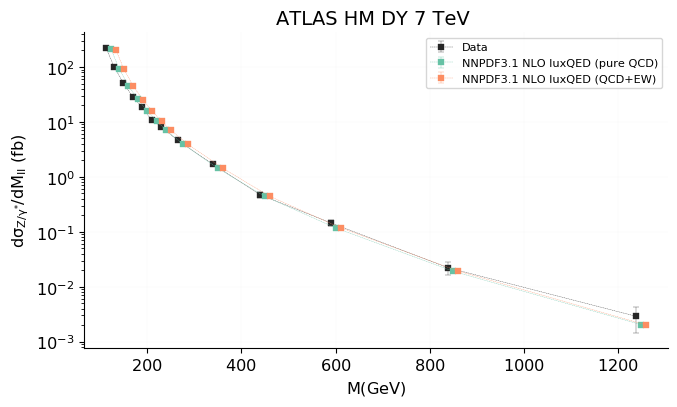
\includegraphics[width=0.5\textwidth]{plots/matched_datasets_from_dataspecs0_plot_fancy_dataspecs_0}
    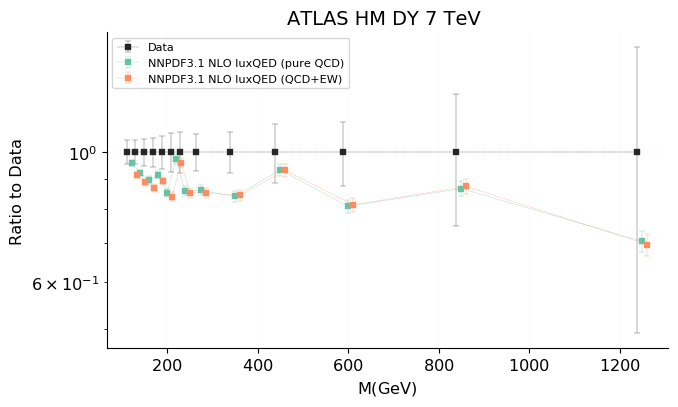
\includegraphics[width=0.5\textwidth]{plots/matched_datasets_from_dataspecs0_datanorm_plot_fancy_dataspecs_0}
    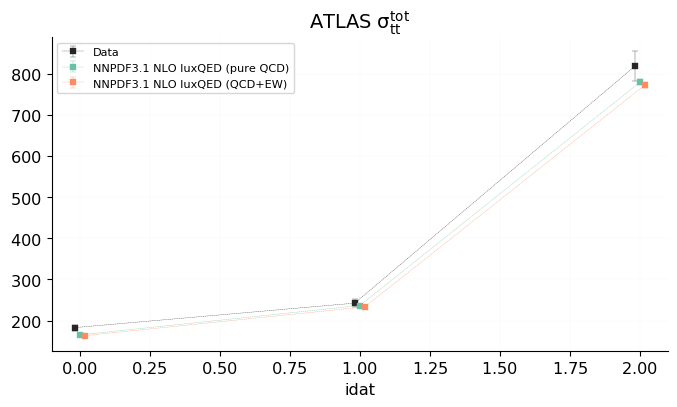
\includegraphics[width=0.5\textwidth]{plots/matched_datasets_from_dataspecs1_plot_fancy_dataspecs_0}
    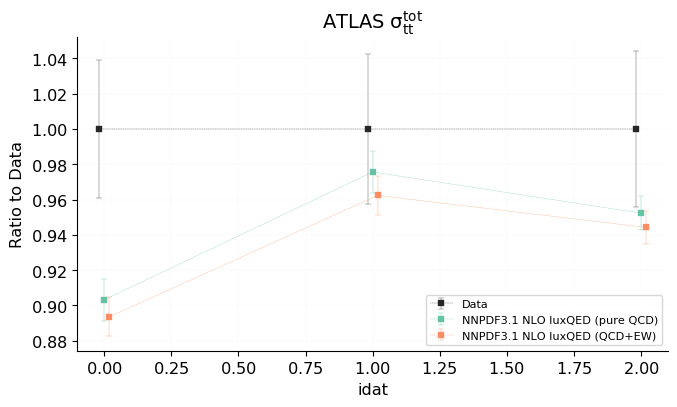
\includegraphics[width=0.5\textwidth]{plots/matched_datasets_from_dataspecs1_datanorm_plot_fancy_dataspecs_0}
    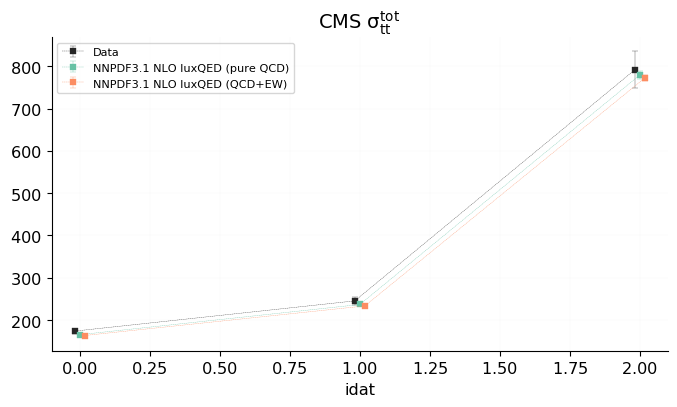
\includegraphics[width=0.5\textwidth]{plots/matched_datasets_from_dataspecs2_plot_fancy_dataspecs_0}
    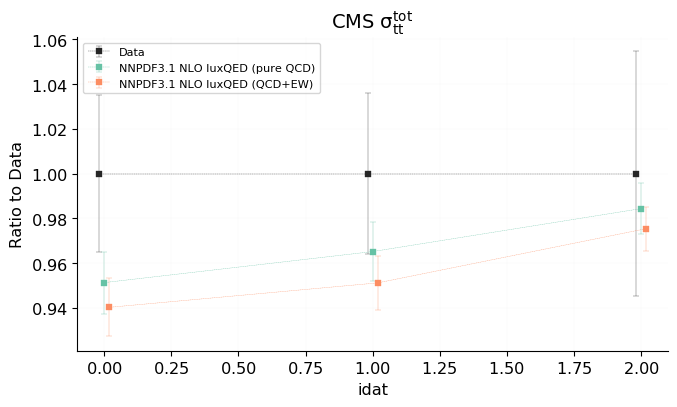
\includegraphics[width=0.5\textwidth]{plots/matched_datasets_from_dataspecs2_datanorm_plot_fancy_dataspecs_0}
    \caption{Data prediction comparison plots.}
    \label{fig:datacomparison}
\end{figure}

\section{Double counting}

Count von Count, ALL

Explain the problem to experimentalists.\\

\section{Outlook}

ALL

\cite{Carli:2010rw}
\cite{Bertone:2014zva}

\appendix

\acknowledgments

S.C. and C.S. are supported by the European Research Council under the European Unions Horizon 2020 research and innovation Programme (grant agreement no. 740006).

\section{More details about \texorpdfstring{\textsc{PineAPPL}}{PineAPPL}}
\label{app:pineappl-interface}

\input{pineappl-appendix}

\bibliographystyle{JHEP}
\bibliography{paper}

\end{document}
